\documentclass[11pt]{article}
\usepackage{mypackages}
\begin{document}

\section{Improving policies}

Now that we can update and maintain an estimator of the value function, we want
to focus on improving our policy.
As something new, we learn the policy as a parameterized function $\pi(a, s, \theta_t)$
with weight $\theta_t$, which given an action $a$ and a state $s$ returns the probability
of taking action $a$ in state $s$.
The goal of the learning agent is to find the best policy, as this is the one
that will maximize the expected return by definition.
To examine how well a policy is doing, we use a \textit{performance measure}, $\rho(\theta_t)$, to evaluate
the policy based on the policy weights $\theta_t$.
We want to maximize the performance measure, since the policy is then optimal with
respects to $\rho(\theta_t)$, so just like in section \ref{sec:td}
we perform gradient ascent to find the optimal weights of the performance measure.
Thus, the update of the policy weights is defined as
\begin{equation}
    \theta_{t+1} = \theta_t + \alpha \nabla_{\theta_t} \rho(\theta_t)
\end{equation}
where $\alpha$ is a parameter determining how large steps we take in our gradient ascent.

We want the performance measure to favor actions that are rarely taken, so that
their contribution to the weights are the same as that of the actions that are
taken more often.
This means that a larger gradient step should be taken if there was a small probaility
of sampling the action from the probability, from which the following performance
measure can be constructed
\begin{equation}
    \begin{aligned}
        \rho(\theta_t) & = \log\pi(a|s, \theta_t)
    \end{aligned}
\end{equation}

The reason for choosing such a performance measure is that
\begin{equation}\label{per_mes}
    \begin{aligned}
        \nabla_{\theta_t} \log\pi(a|s, \theta_t) = \frac{\nabla_{\theta_t}\pi(a|s, \theta_t)}{\pi(a|s,\theta)}
    \end{aligned}
\end{equation}
which means a low probability increases the magnitude of the gradient
in such a way that over time, all actions should be able to influence the
weights the same.

The environments used in this project all have a continuous state space,
and a discrete action space.
This means that there is a possibility of the policy turning deterministic,
which is a problem because the learning agent won't be exploring the environment anymore
and because our performance measure from equation \ref{per_mes} only works for
non-deterministic policies.

We can solve this problem by choosing our policy in a way that doesn't allow probabilities that are 0 or 1.
In this project we will be using the \textit{softmax} function to achieve this,
by using a numerical preference $h(s, a, \theta) \in \mathbb{R}$
for each action available from the state $s$.
This means that the softmax function over the numerical preferences can be used as a policy
as shown in equation \ref{eq:soft_max}.
\begin{equation}\label{eq:soft_max}
    \pi(a | s, \theta_t) = \frac{e^{h(s,a,\theta_t)}}{\sum\limits_{a} e^{h(s,a,\theta_t)}}
\end{equation}

\subsection{The Actor-Critic model}

In this next step we want to combine the use of both a parameterized value function, $\hat{v}(s, \mathbf{w}_t)$,
and a parameterized policy, $\pi(a|s, \theta_t)$.
A problem with the performance measure from equation \ref{per_mes} is that
the updates doesn't depend on the rewards received through the game.
To avoid updating without taking the rewards into account, we can
use the value function to evaluate the policy.
This means that after an action sampled from $\pi(a|s,\theta)$ is performed,
the reward following the action is used by the value function to
compute the one-step TD-error from section \ref{sec:td}.
\begin{equation*}
    \delta_t =  R_t + \gamma \hat{v} (S_{t+1}, \mathbf{w_t}) - \hat{v}(S_t, \mathbf{w_t})
\end{equation*}
We can use this error to update the weights of the policy, as
a way to weigh the performance measure - if the TD-error is low,
the gradient step should be small, and vice versa.
\begin{equation}
    \theta_{t+1} = \theta_t + \delta_t \nabla_{\theta} \log \pi(A | S, \theta)
\end{equation}
This way of using the value function and policy is called an
\textit{Actor-Critic} method, where the policy can be seen as an actor
which is able to interact with the environment, while the value function
is the critic, evaluating the actions of the actor and thus
influencing the policy indirectly.

\begin{figure}[!h]
    \centering
    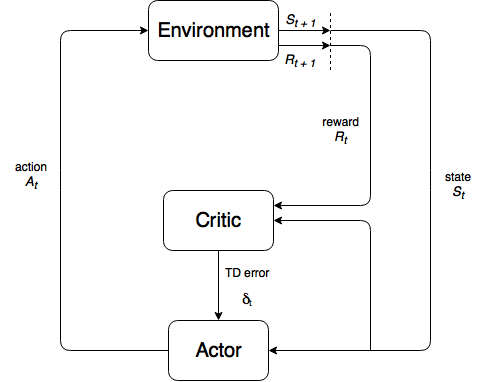
\includegraphics[scale = 0.5]{include/ActorCriticDiagram.png}
    \caption{A representation of the workflow in an Actor-Critic
    model. The environment sends a state and reward signal to both the actor and the critic. The critic compute the TD-error which is sent to the actor,
and then the actor perform a action and so forth.}
    \label{fig:actor-critic}
\end{figure}
%An advantage of using Actor-Critic methods is that the split into a actor and critic, reduces the variance of the function approximation, because the update step size for the policy parameters is defined relative to estimated value from critic.\cite{actCrit}


\subsection{Actor-Critic with Eligibility Traces}

In this project we using the \textit{Actor-Critic with eligibility traces}, which follow the workflow from figure \ref{fig:actor-critic}, and using eligibility traces for performing online updates of the weight vectors $\theta$ and $\mathbf{w}$. The general updating scheme for the eligibility vector $\mathbf{e}^{\mathbf{w}}$ is,
\begin{equation}
    \mathbf{e}^{\mathbf{w}} \leftarrow \lambda^{\mathbf{w}} \mathbf{e}^{\mathbf{w}} + \nabla_{\mathbf{w}} \hat{v}(S, \mathbf{w})
\end{equation}
and $\mathbf{e}^{\theta}$ as,
\begin{equation}
    \mathbf{e}^{\theta} \leftarrow \lambda^{\theta} \mathbf{e}^{\theta} + \nabla_{\theta} \text{log} \pi (A | S, \theta)
\end{equation}
where $\lambda$ discussed in section \ref{sec:eligibility_traces} is the discount rate, there represent how much the existing eligibility trace influence the update.
\\
By using eligibility traces in Acotr-Critic methods we can keep information of how the gradients have changed in the last minor time period. The reason that is smart to use these eligibility traces is that we can update the parameters based on the trend of how the parameters have changed in the last time, for both the weight vector $\mathbf{w}$,
\begin{equation}
    \mathbf{w} \leftarrow \mathbf{w} + \beta \delta \mathbf{e}^{\mathbf{w}}
\end{equation}
and $\theta$,
\begin{equation}
    \theta \leftarrow \theta + \alpha \delta \mathbf{e}^{\theta}
\end{equation}
where $0 \leq \alpha \leq 1$ and $0 \leq \beta \leq 1$ is the step-size parameters, which defines how much the eligibility traces influence the update. 

We have implemented Actor-Critic with eligibility traces to solve the CartPole problem, which we will discuss in section KOM MED REF, using the algorithm from Appendix \ref{sec:pseudo_code_et}








%\printbibliography
%\bibliography{citations}
%\bibliographystyle{plain}
\end{document}
